\section{Chapter 4}

	In this chapter, future projects are discussed. Some of these projects stem from unanswered questions in previous work, while some of them will be completely new.
	
	\subsection{Power law scaling of entanglement peak in the $tV$ model}
	
	%%%%%%%%%%
	\begin{figure}[h]
	\begin{center}
	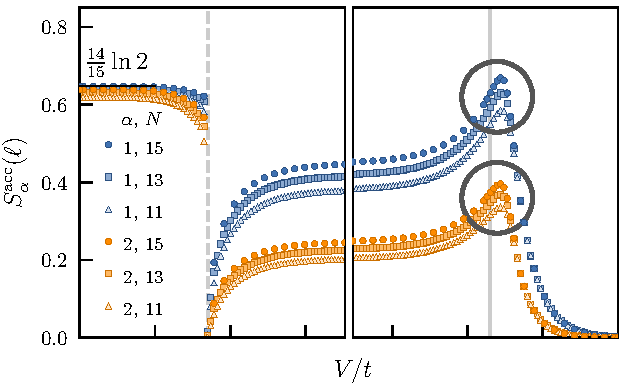
\includegraphics[scale=1.0]{operationalEntanglementEntropies_SOP5_withPeakCircles.pdf}
	\end{center}
	\caption{Accessible entanglement entropies as a function of interaction strength in the $t-V$ model. The circles enclose a region where both the von Neumann and R\'enyi entanglement entropies attain a maximum value. As the total number of particles $N$ increases, this maximum seems to be shifting to the left, closer to the phase transition $V/t=2$.}
	\label{fig:OEE_circledPeaks}
	\end{figure}
	%%%%%%%%%%
	
	In the $t-V$ model, there are two known phase transitions, a first order one at $V/t=-2$, and a continuous one at $V/t=2$. From Figure \ref{fig:OEE_circledPeaks}, it can be seen that the accessible entanglement entropies are sensitive to both types of transition. Interestingly, this sensitivity to the transition in $V/t=2$ expresses itself as a peak of entanglement. Moreover, the interaction strength at which this peak of entanglement occurs moves closer to the exact value of the continuous phase transition as the number of particles in the system increases.  
	
	%%%%%%%%%%
	\begin{figure}[h!]
	\begin{center}
	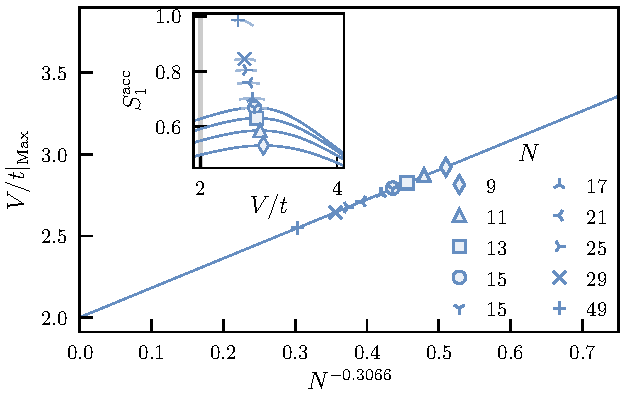
\includegraphics[scale=1.0]{peakScalingOddN.pdf}
	\end{center}
	\caption{Interaction strength at which the maximum $S_{1}^{\mathrm{acc}}$ occurs as a 	function of the total number of particles $N$. The exponent of $N$ was obtained from a l	inear fitting of $\ln N$ vs. $\ln{(V/t - 2)}$.  Although very few points are plotted due to 	memory limitations, they agree with the hypothesis that for $N \to \infty$, the peak of 	von Neumann accessible entanglement occurs at the phase transition $V/t = 2$. Inset: 	$S_{1}^{\mathrm{acc}}$ as a function of interaction strength $V/t$ for various $N$ 		around the neighborhood of the peak.}
	\label{fig:peakScalingOddN}
	\end{figure}
	%%%%%%%%%%
	
	Figure \ref{fig:peakScalingOddN} shows the value where the entanglement peak occurs for various system sizes. The fact that all the points lie on a line that intercepts the vertical axis at $V/t_{Max}=2$ is very promising. Nevertheless, the current scaling exponent of $-0.2545$ should not be taken for granted due to how small the systems currently are. Indeed, the continuous phase transition should occur in the $t-V$ model at $V/t=2$, but this is for a system where $N \to \infty$. More data points, corresponding to large systems are still be needed to get closer to this intercept and confirm the power law scaling.	

	
	\subsection{Filling fraction dependence of entanglement}
	
	The $t-V$ model results presented in this thesis were focused on the special case of half filling. That is, only half of the lattice sites were had particles in them ($N = L/2$). For this case, the exact results for the phase transitions are mapped from the XXZ spin-$1/2$ model. For other filling fraction, a theory has yet to be developed. Figure \ref{fig:fillingFractionDependence} shows the accessible entanglement entropies for various filling fractions ranging from $1/14$ to $1/2$. 
	
	%Figure 8
	%%%%%%%%%%
	\begin{figure}[h!]
	\begin{center}
	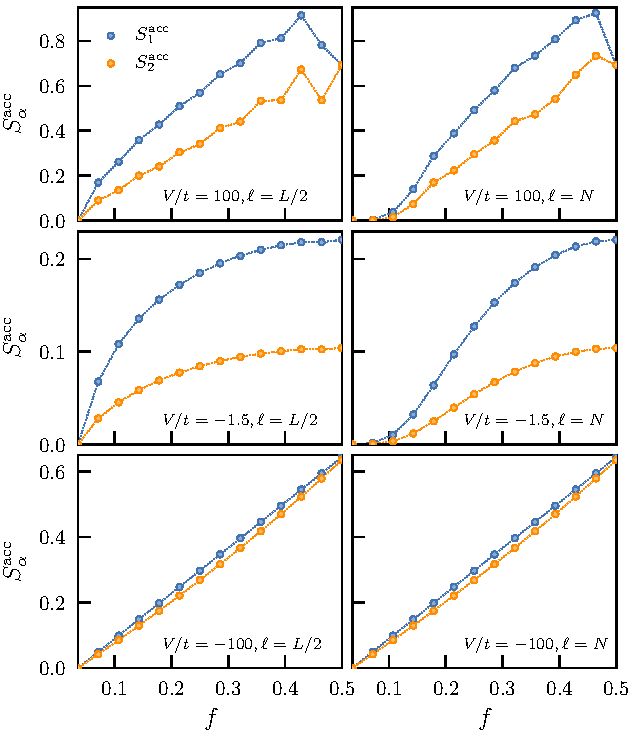
\includegraphics[scale=1.0]{fillingFractionDependence.pdf}
	\end{center}
	\caption{Accessible entanglement entropies $S_{\alpha}^{\mathrm{acc}}(\ell)$ for $		\alpha = 1,2$ as a function of filling fraction $N/L$. The lattice size was kept fixed at 		$L=28$ sites and the total number of particles were $N=1,2,3...14$. For the left column, 	the spatial partition $\ell$ was kept fixed at half the lattice size, $\ell = L/2$. For the right 	column, it was set to equal the total number of particles $N$. The interaction strengths 	$V/t$ are indicated in each of the plots and correspond to values from each of the three 	phases of the $t-V$ model.}
	\label{fig:fillingFractionDependence}
	\end{figure}
	%%%%%%%%%%
	
	\subsection{Accessible entanglement via quantum gates}
	
	The endgame for the study of accessible entanglement entropies is to exploit the entanglement of a system as a resource. Motivated by this, we are currently working on building a quantum circuit that reproduces the accessible entanglement measurement process. After coming up with the appropriate quantum circuit, the results will be tested on IBM's quantum computer \cite{IBMQuantumExp:2018:Online}.
	
	\subsection{Entanglement in the Bose-Hubbard model}
	
	Another project in the works is calculating accessible entanglement entropies in the Bose-Hubbard (BH) model. In the study of fermionic systems, such as the $t-V$ model, methods like exact diagonalization and density matrix renormalization group must be used to due to the infamous sign problem. The high memory cost of these methods restricts simulations to only relatively small system sizes. Nevertheless, the sign problem non-existent in bosonic models and thus quantum Monte Carlo (QMC) methods can be used. QMC will allow the study of much larger systems than the ones presented here.